\chapter{Interaction design}
\chlab{design}

\begin{comment}
Here will be the interaction designs for the tool\ldots

\nlipsum

\begin{quote}
``Design is an act of choosing among [\ldots] future ways of being''

\leftskip=.5cm-- \textit{Eli Blevis}~\cite{blevis2007sustainable}
\end{quote}
\end{comment}

From the fact that the idea of fragment-based molecule parameterisation is a new concept, it is no surprise that there are no existing tools for this. Furthermore, no tools exist that allow for easy comparison of molecules - or fragments of them - either. What does exist is a wide range of tools and programs for visualising, creating and editing molecules. This includes stand-alone molecule drawing software such as \verb|Accelerys Draw|~\cite{accelrys2012accelrys}, \verb|Avogadro|~\cite{hanwell2012avogadro}, \verb|PyMOL|~\cite{delano2002pymol}, and \verb|RasMol|~\cite{pembroke2000bio}, two-dimensional web based molecule editors like \verb|ChemDoodle 2D Sketcher|~\cite{ichemlabs2013chemdoodle}, \verb|Marvin4JS|~\cite{chemxon2013marvin}, and \verb|Molsoft HTML5 Molecule Editor|~\cite{molsoft2012molsoft}, and online three-dimensional visualisation tools \verb|CanvasMol|~\cite{altered2013canvasmol} and \verb|JSMol|~\cite{hanson2013jsmol}.

These existing tools will serve as an initial guideline for the molecule parameterisation system that is to be developed. Parts of their implementations may be reused, or could provide some inspiration on how to implement those parts in the new system. The rest of the tool, however, will need to be designed and developed from scratch.

This chapter will discuss interaction design for a fragment-based molecule parameterisation system. The design will follow the basic interaction design principles as posed by Norman and others~(see \secref{id_principles}), the knowledge about learing~(see \secref{id_learning}), and keep in mind the insights gained by the developers of other molecule software~(see \secref{software}). This way, the system should be able to meet its requirements that have been stated in \chref{analysis}.


\section{Platform}
Over the past few years, there has been a trend in bringing everything to the web~\cite{ertl2010molecular}. This includes several molecule software packages, such as \verb|JSMol|~\cite{hanson2013jsmol} and \verb|JSME|~\cite{bienfait2013jsme}~(see also \secref{software}). Following this trend, it has been decided to implement the front-end of the molecule parameterisation system using \verb|HTML5|, \verb|CSS3| and \verb|JavaScript|. This allows for great portability and availability across different operating systems and platforms.

Having the user interface as a web service means that the back-end, where the actual finding of matching fragments occurs, also needs to be available through the web. For this purpose, the choice has been made to use the \verb|Python| web framework \verb|Django| for that part. This framework can easily be set up on various platforms and provides a wide span of features.


\section{Two versions}
As there is no existing software for fragment-based molecule parameterisation, there is also no baseline to which the developed tool can be compared. In order to still be able to say something about the quality of the tool, two different implementations of it will be made. There are a few axes along which this difference can be made. One could, for instance, compare two tools that have different visualisation methods. Visualising molecules, however, is a well-exhausted field of research, leaving very little room for new ideas. Furthermore, it is not even possible to represent molecules in textual form here, as a visual representation is essential to perceive similarity of fragments~\cite{gallopoulos1994computer}.

Another possible variable in the tool is the way its users will interact with it and especially its degree of automation. Varying this degree has been the subject of several studies~(e.g.~\cite{payne2000varying, horvitz1999principles, marcus1987taking, norman1990problem}, see also \secref{id_automation}), all of which concluded the degree to which automation can be applied is highly dependent on the context of the system and sometimes even to the situation in which the system is used.

When implementing multiple versions of a tool with different levels of automation, it is often decided to make three versions: a `naive' version without much automation, a `cooperative' version in which the user is given advise, and an `autonomous' version that only requires some parameterisation~(see~\cite{payne2000varying} and \secref{id_automation}). As it is considered hard to parameterise a molecule based on fragments of other molecules and little is known on what is the best way of doing this, an autonomous version of a tool that does this cannot yet be developed. The other two versions, however, seem to be perfectly implementable and both can be considered useful.

\begin{figure}[h!]
\begin{center}
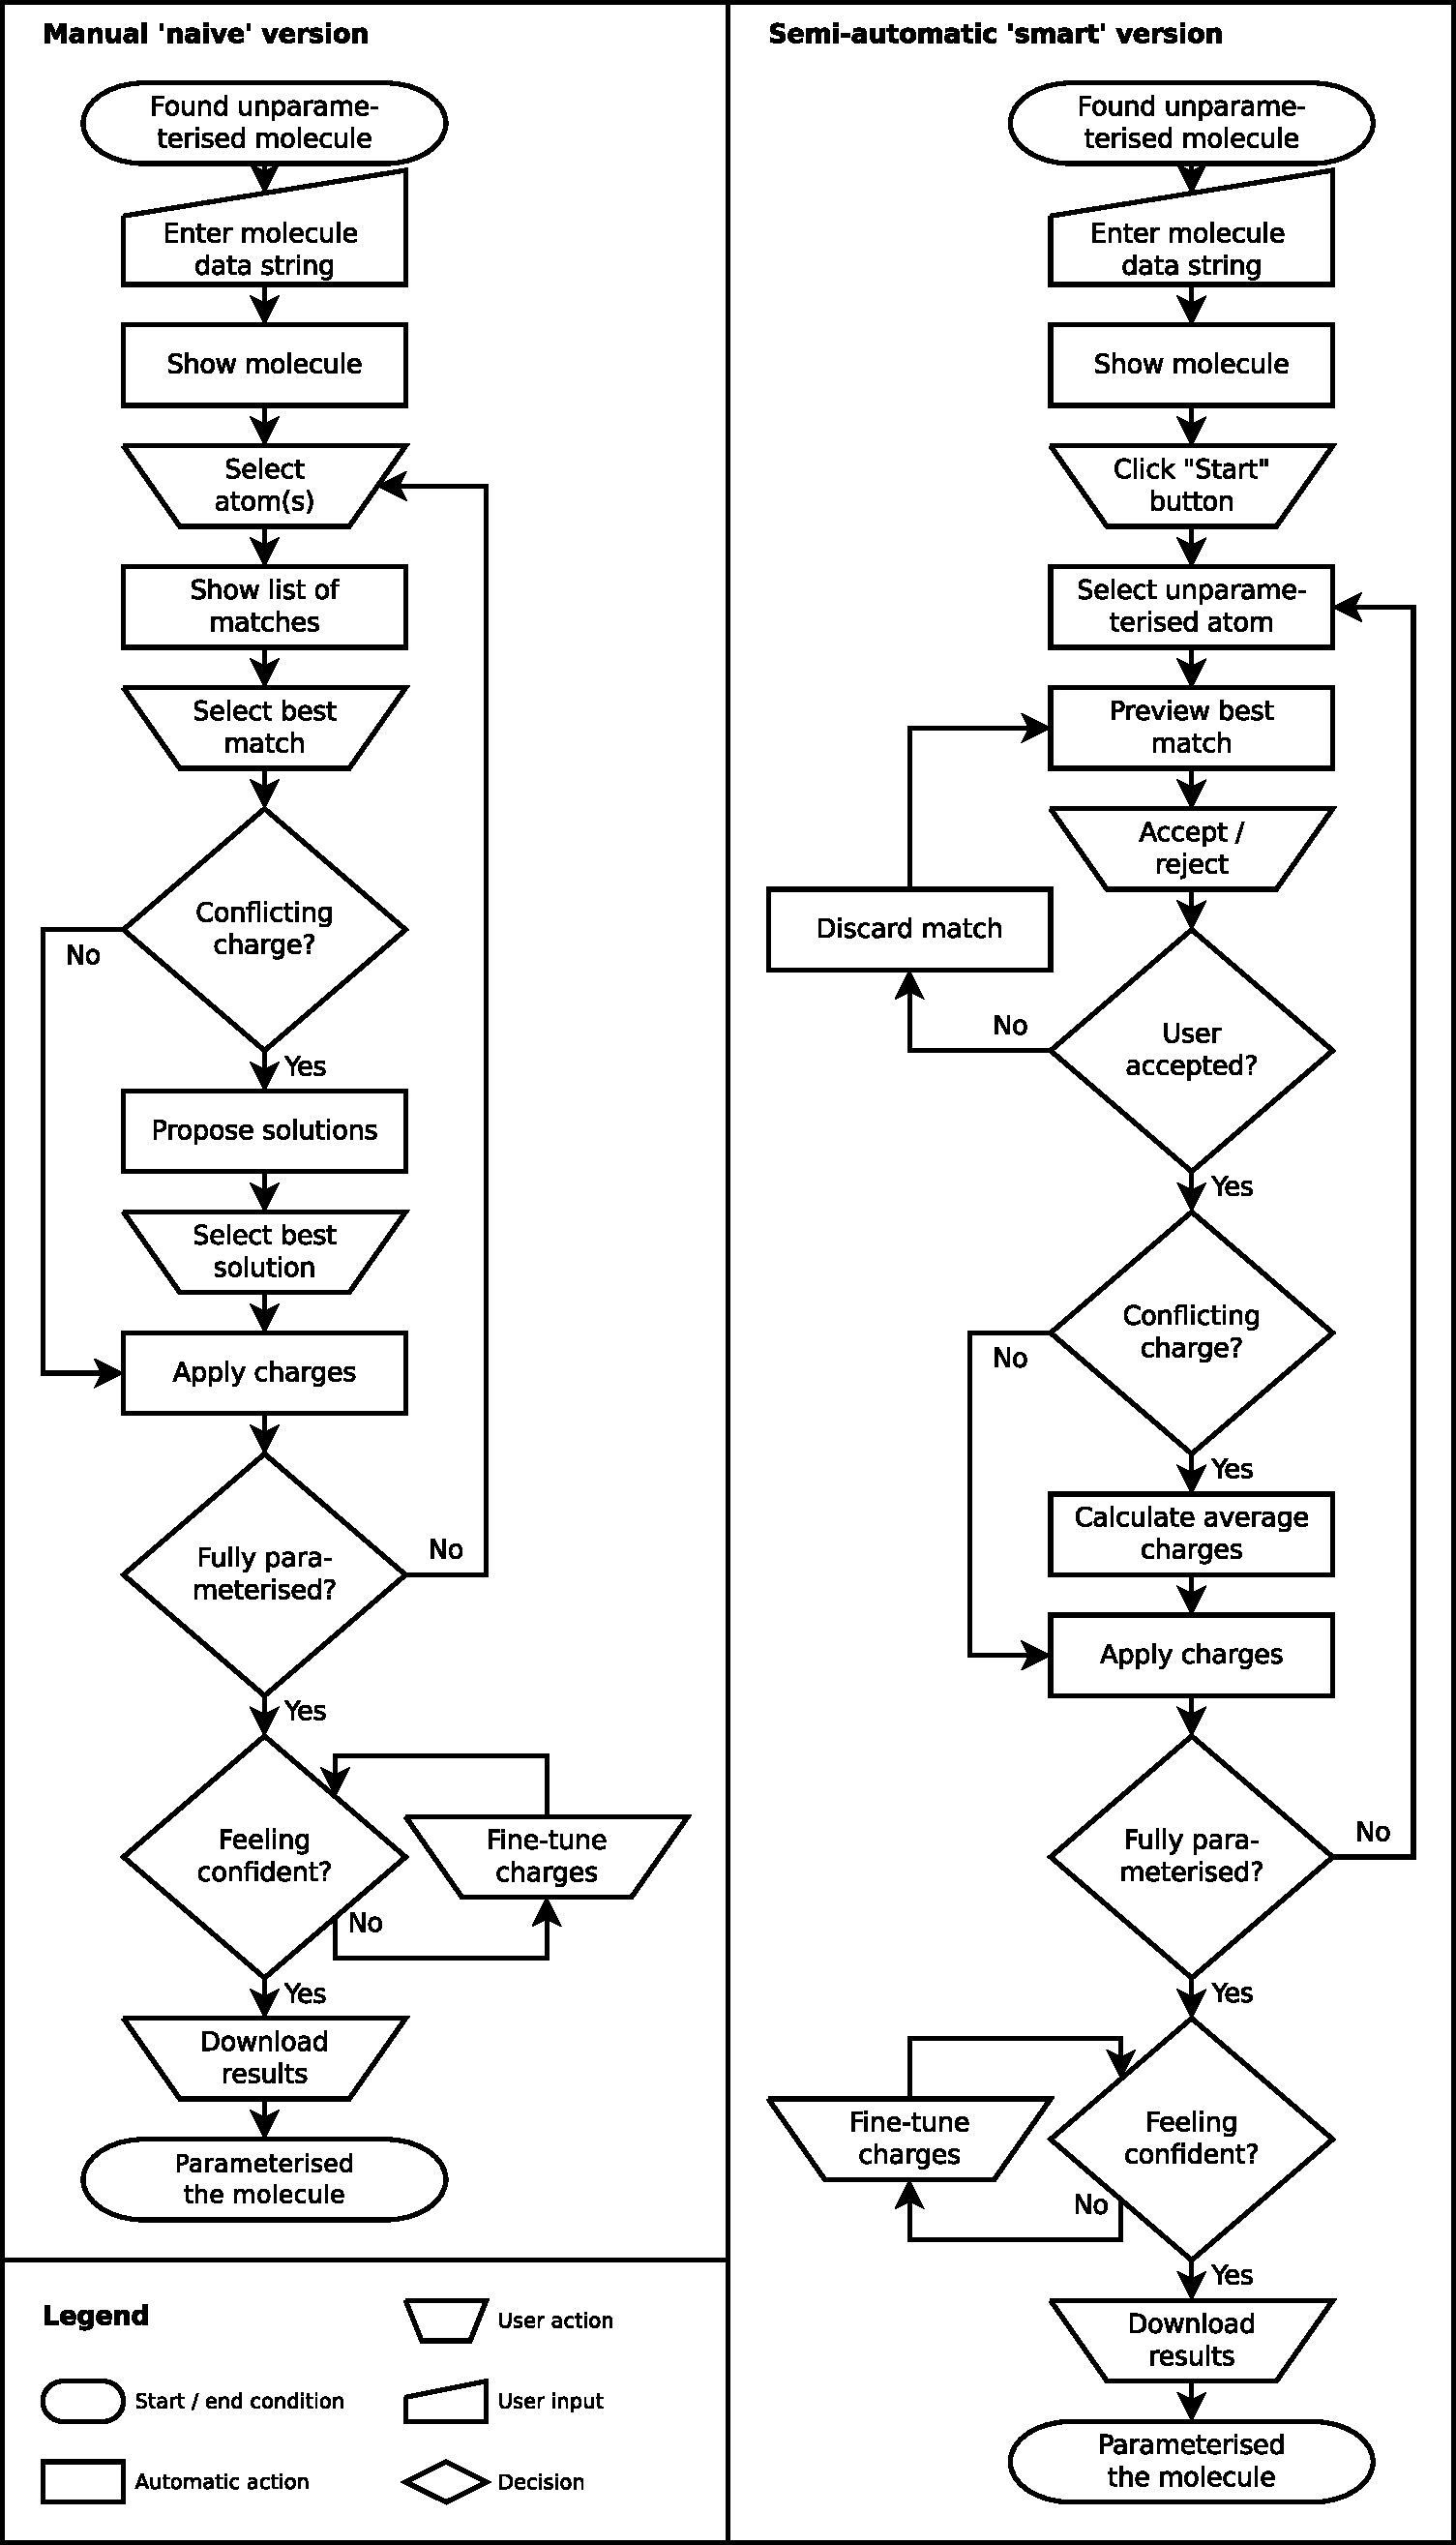
\includegraphics[width=.9\textwidth]{img/complete_id.pdf}
\caption{The two different interaction designs.}
\figlab{id_flows}
\vspace{-2cm}
\end{center}
\end{figure}

\Figref{id_flows} shows a naive and a cooperative interaction design for the tool that will be developed. Here, the cooperative design has been called the `smart' version to accentuate its differences with the naive version. The following sections will discuss these two interaction designs, the motivation behind them, and their workings.

\subsection{Commonalities}
As can be seen in \figref{id_flows}, the two interaction designs share a common start and ending. First of all, the user will need to find a molecule which he wishes to parameterise. That molecule then needs to be inserted into the system. For that purpose, the user needs to find a representation of the molecule that the system can work with. It has been decided that this so called molecule data string needs to be in the \verb|SMILES|~\cite{daylight1992daylight}, \verb|InChI|~\cite{heller2013inchi}, or \verb|PDB|~\cite{bernstein1977protein} format, as these are the most commonly used.

As many users of the system will be users of the ATB and will probably also find the molecules they want to use the molecule parameterisation system for in the ATB repository, it is should also be possible to submit an \verb|ATB molecule ID|. From that, the system should automatically retrieve the \verb|PDB| structure file that is stored on the ATB servers. This can then be used to get the atom positions and display the molecule to the user.

After the molecule has been shown to the user, the two versions of the interaction design start to differ. This will be discussed in more detail in the following sections, where \secref{id_naive} discusses the `naive' version, and \secref{id_smart} describes the `smart' interaction design.

After the molecule has completely been parameterised, the two interaction designs join the same path once more. The user now has the possibility to manually fine-tune the charges, if he feels that this is needed. This can be done by selecting an atom and clicking an ``Edit charge'' button. In order to assist the user in finding a proper charge for the atom, the molecule fragments that have been used to get the current charge can be displayed. As soon as the user feels the assigned charges are correct, he should be able to download a file containing the results of the parameterisation.

In order to reduce the effect of user mistakes on the parameterisation process, every user action can be undone. If something has accidentally been undone, it can also be redone using a ``Redo'' button. This way, the user does not need to start over completely when he makes a small mistake, such as accidentally selecting the wrong fragment. It also allows for more experimentation, as there are no definitive consequences of any user action.


\subsection{Manual `naive' version}
\seclab{id_naive}
Just like the naive RPA implementation from~\cite{payne2000varying}, the only automatic process occurring in the naive version of the molecule parameterisation tool is the validation of user input. Besides ordering the matching fragments based on their probability of being a good match, the tool will not give any advise, nor will it automatically infer any values.

\subsubsection{Operation}
The operation of the naive version of the tool is shown in \figref{id_flows}. In more detail, the complete set of steps required to fully parameterise a molecule is as follows:
\begin{enumerate}[itemsep=.1em, parsep=.2em, topsep=0em]
\item The user enters a molecule data string (in \verb|SMILES|, \verb|InChI|, \verb|PDB| format, or using an \verb|ATB molecule ID|). The molecule will be displayed to the user;
\item The user selects a single atom or a group of \emph{connected} atoms. They need to be connected, since non-connected atoms do not affect each other;
\item A list of matching fragments will be loaded shown, ordered such that the highest rated match comes first and the lowest last. The user can browse through them, preview the result of selecting that match and, once he has found what he sees as the best match, select this match;
\item
  \begin{itemize}[leftmargin=0cm, itemsep=.1em, parsep=.1em]
  \item[]{\bf Fragment contains parameterised atoms}:
    \begin{enumerate}
    \item
      Details of the charge conflict are shown, along with the a list of possible solutions. The user picks one of the following solutions:
      \begin{itemize}[itemsep=.1em, parsep=.2em, topsep=0em]
      \item Take the average of the two charges;
      \item Keep the current value;
      \item Take the new value;
      \item Manually enter a value.
      \end{itemize}
    \item The solution is applied and the resulting charges are assigned to the molecule.
    \end{enumerate}
  \item[] {\bf Fragment only contains unparameterised atoms}:\\
    The charges from that fragment are assigned to the molecule;
  \end{itemize}
\item
  \begin{itemize}[leftmargin=0cm, itemsep=.1em, parsep=.1em]
  \item[]{\bf Unparameterised atoms remain}:\\The user selects another atom / list of connected atoms. Back to step 2;
  \item[] {\bf Molecule fully parameterised}:\\Continue to step 6;
  \end{itemize}
\item
  \begin{itemize}[leftmargin=0cm, itemsep=.1em, parsep=.1em]
  \item[] {\bf User feels charges need to be fine-tuned}:
    \begin{enumerate}
    \item The user selects the atom which' charge he wants to modify;
    \item The user clicks the ``Edit charge'' button for that atom;
    \item The user can now view the fragments that were used to find the charge for this molecule. Using that and potentially other information, he can find a better charge for the atom.
    \item The user enters the improved charge in an input field and clicks the ``Apply charge'' button. The charge will be assigned to the atom;
    \item Re-evaluate the conditions of step 6.
    \end{enumerate}
  \item[]{\bf User feels satisfied}:\\Continue to step 7;
  \end{itemize}
\item The user can now download the result of the parameterisation process. After he has done this, the process has been completed.
\end{enumerate}

\subsubsection{Motivation}
As pointed out earlier, it is important to have a non-automatic baseline to see if automation can work for a certain tool. This naive version can serve as that baseline. In this case, however, it might even serve as more than just a baseline. It could also quite possibly be a better fit for the molecule parameterisation task than any automated version. The same was concluded for the naive RPA in~\cite{payne2000varying}, which was largely outperformed by its more automated siblings, but offered great benefits in situations where full control was required.

In the naive molecule parameterisation tool, the user can manually decide what atoms need to be parameterised and has a clear overview of all matching fragments. Furthermore, he can manually decide what should happen with overlapping fragments and can modify atom charges at any point in the process. This provides the same benefits as the previously discussed naive RPA had.

Another reason why this naive version might work better than an automated one is the fact that this one encourages exploring different options. By providing a list of fragments, rather than proposing a single one, the fragments can easily be compared such that the chances for the best match being selected increase. Furthermore, as the user is free to determine what atoms should be parameterised at which point in time and is also able to select groups of atoms, he can experiment with the selection size and order, which may lead to better results.


\subsection{Semi-automatic `smart' version}
\seclab{id_smart}
Inspired on the cooperative RPA from~\cite{payne2000varying}, \verb|LookOut|~\cite{horvitz1999principles}, and \verb|SALT|~\cite{marcus1987taking}, the smart tool for molecule parameterisation will continuously make suggestions to the user. After the parameterisation process has been started, the system will continuously propose fragments to the user, which he only needs to accept or reject.

\subsubsection{Operation}
The operation of the smart version of the tool is shown in \figref{id_flows}. In more detail, the complete set of steps required to fully parameterise a molecule is as follows:
\begin{enumerate}[itemsep=.1em, parsep=.2em, topsep=0em]
\item The user enters a molecule data string (in \verb|SMILES|, \verb|InChI|, \verb|PDB| format, or using an \verb|ATB molecule ID|). The molecule will be displayed to the user;
\item The user clicks the ``Start parameterising'' button. One of the atoms on the edge of the molecule will now be automatically selected and matching fragments for it will be retrieved;
\item The highest rated match is previewed on the molecule. The user can either accept or reject this proposed match;
\item
  \begin{itemize}[leftmargin=0cm, itemsep=.1em, parsep=.1em]
  \item[]{\bf Rejected}:\\Remove this match from the list of matching fragments (the user \emph{can} go back to this one if he changes his mind). Back to step 3;
  \item[] {\bf Accepted}:
    \begin{itemize}[leftmargin=.5cm, itemsep=.1em, parsep=.1em]
    \item[]{\bf Fragment contains parameterised atoms}:\\
      The average of the current and fragment charges is calculated and the resulting charges are assigned to the molecule;
    \item[] {\bf Fragment only contains unparameterised atoms}:\\
      The charges from that fragment are assigned to the molecule;
    \end{itemize}
  \end{itemize}
\item
  \begin{itemize}[leftmargin=0cm, itemsep=.1em, parsep=.1em]
  \item[]{\bf Unparameterised atoms remain}:\\Another unparameterised atom, preferably neighbouring an already parameterised one, is automatically selected and similar fragments are retrieved. Back to step 3;
  \item[] {\bf Molecule fully parameterised}:\\Continue to step 6;
  \end{itemize}
\item
  \begin{itemize}[leftmargin=0cm, itemsep=.1em, parsep=.1em]
  \item[] {\bf User feels charges need to be fine-tuned}:
    \begin{enumerate}
    \item The user selects the atom which' charge he wants to modify;
    \item The user clicks the ``Edit charge'' button for that atom;
    \item The user can now view the fragments that were used to find the charge for this molecule. Using that and potentially other information, he can find a better charge for the atom.
    \item The user enters the improved charge in an input field and clicks the ``Apply charge'' button. The charge will be assigned to the atom;
    \item Re-evaluate the conditions of step 6.
    \end{enumerate}
  \item[]{\bf User feels satisfied}:\\Continue to step 7;
  \end{itemize}
\item The user can now download the result of the parameterisation process. After he has done this, the process has been completed.
\end{enumerate}

\subsubsection{Motivation}
One of the most important reasons for developing a tool for fragment-based molecule parameterisation is to speed up the current process that uses quantum mechanical calculations. Having some automation in this tool can help increasing this benefits even further. By suggesting molecule fragments, parameterising a molecule can potentially be done a lot faster than when the user has to manually go through a list of fragments.

By automating certain parts of the parameterisation process, the tool should also be easier to use. One basically only needs to say `yes' or `no' a few times and will therefore be easy to learn. This increases the potential for new people to start using the tool, thereby enhancing its value. Furthermore, it makes sure users do not get lost in a long list of features. Otherwise, users might make the wrong decisions or even stop parameterising completely~\cite{norman2002design}~(see also \secref{design}).

In order to mediate the often occurring problems with automation, the fine-tuning step at the end has been added, based on studies by Norman~\cite{norman1990problem} and Horvitz~\cite{horvitz1999principles}. As there will always be errors in the automatic charge corrections, this provides the user with a way to identify and improve incorrectly assigned atom charges. Providing the user with the means he needs to see how every charge came to be helps him to determine how that charge can be improved.


\subsection{Comparison}
In order to be able to compare and discuss visual interfaces at an abstract level, Brehmer and Munzner have developed a multilevel typology for abstract visualisation tasks~\cite{brehmer2013multi}~(see also \secref{id_abstraction}). The Brehmer-Munzner typologies\footnote{They have not officially been named, but will be referred to as a `Brehmer-Munzner typology' in the remainder of this document.} for the two implementations of the molecule parameterisation tool are shown in \figref{id_typologies}.

\begin{figure}[h!]
\begin{center}
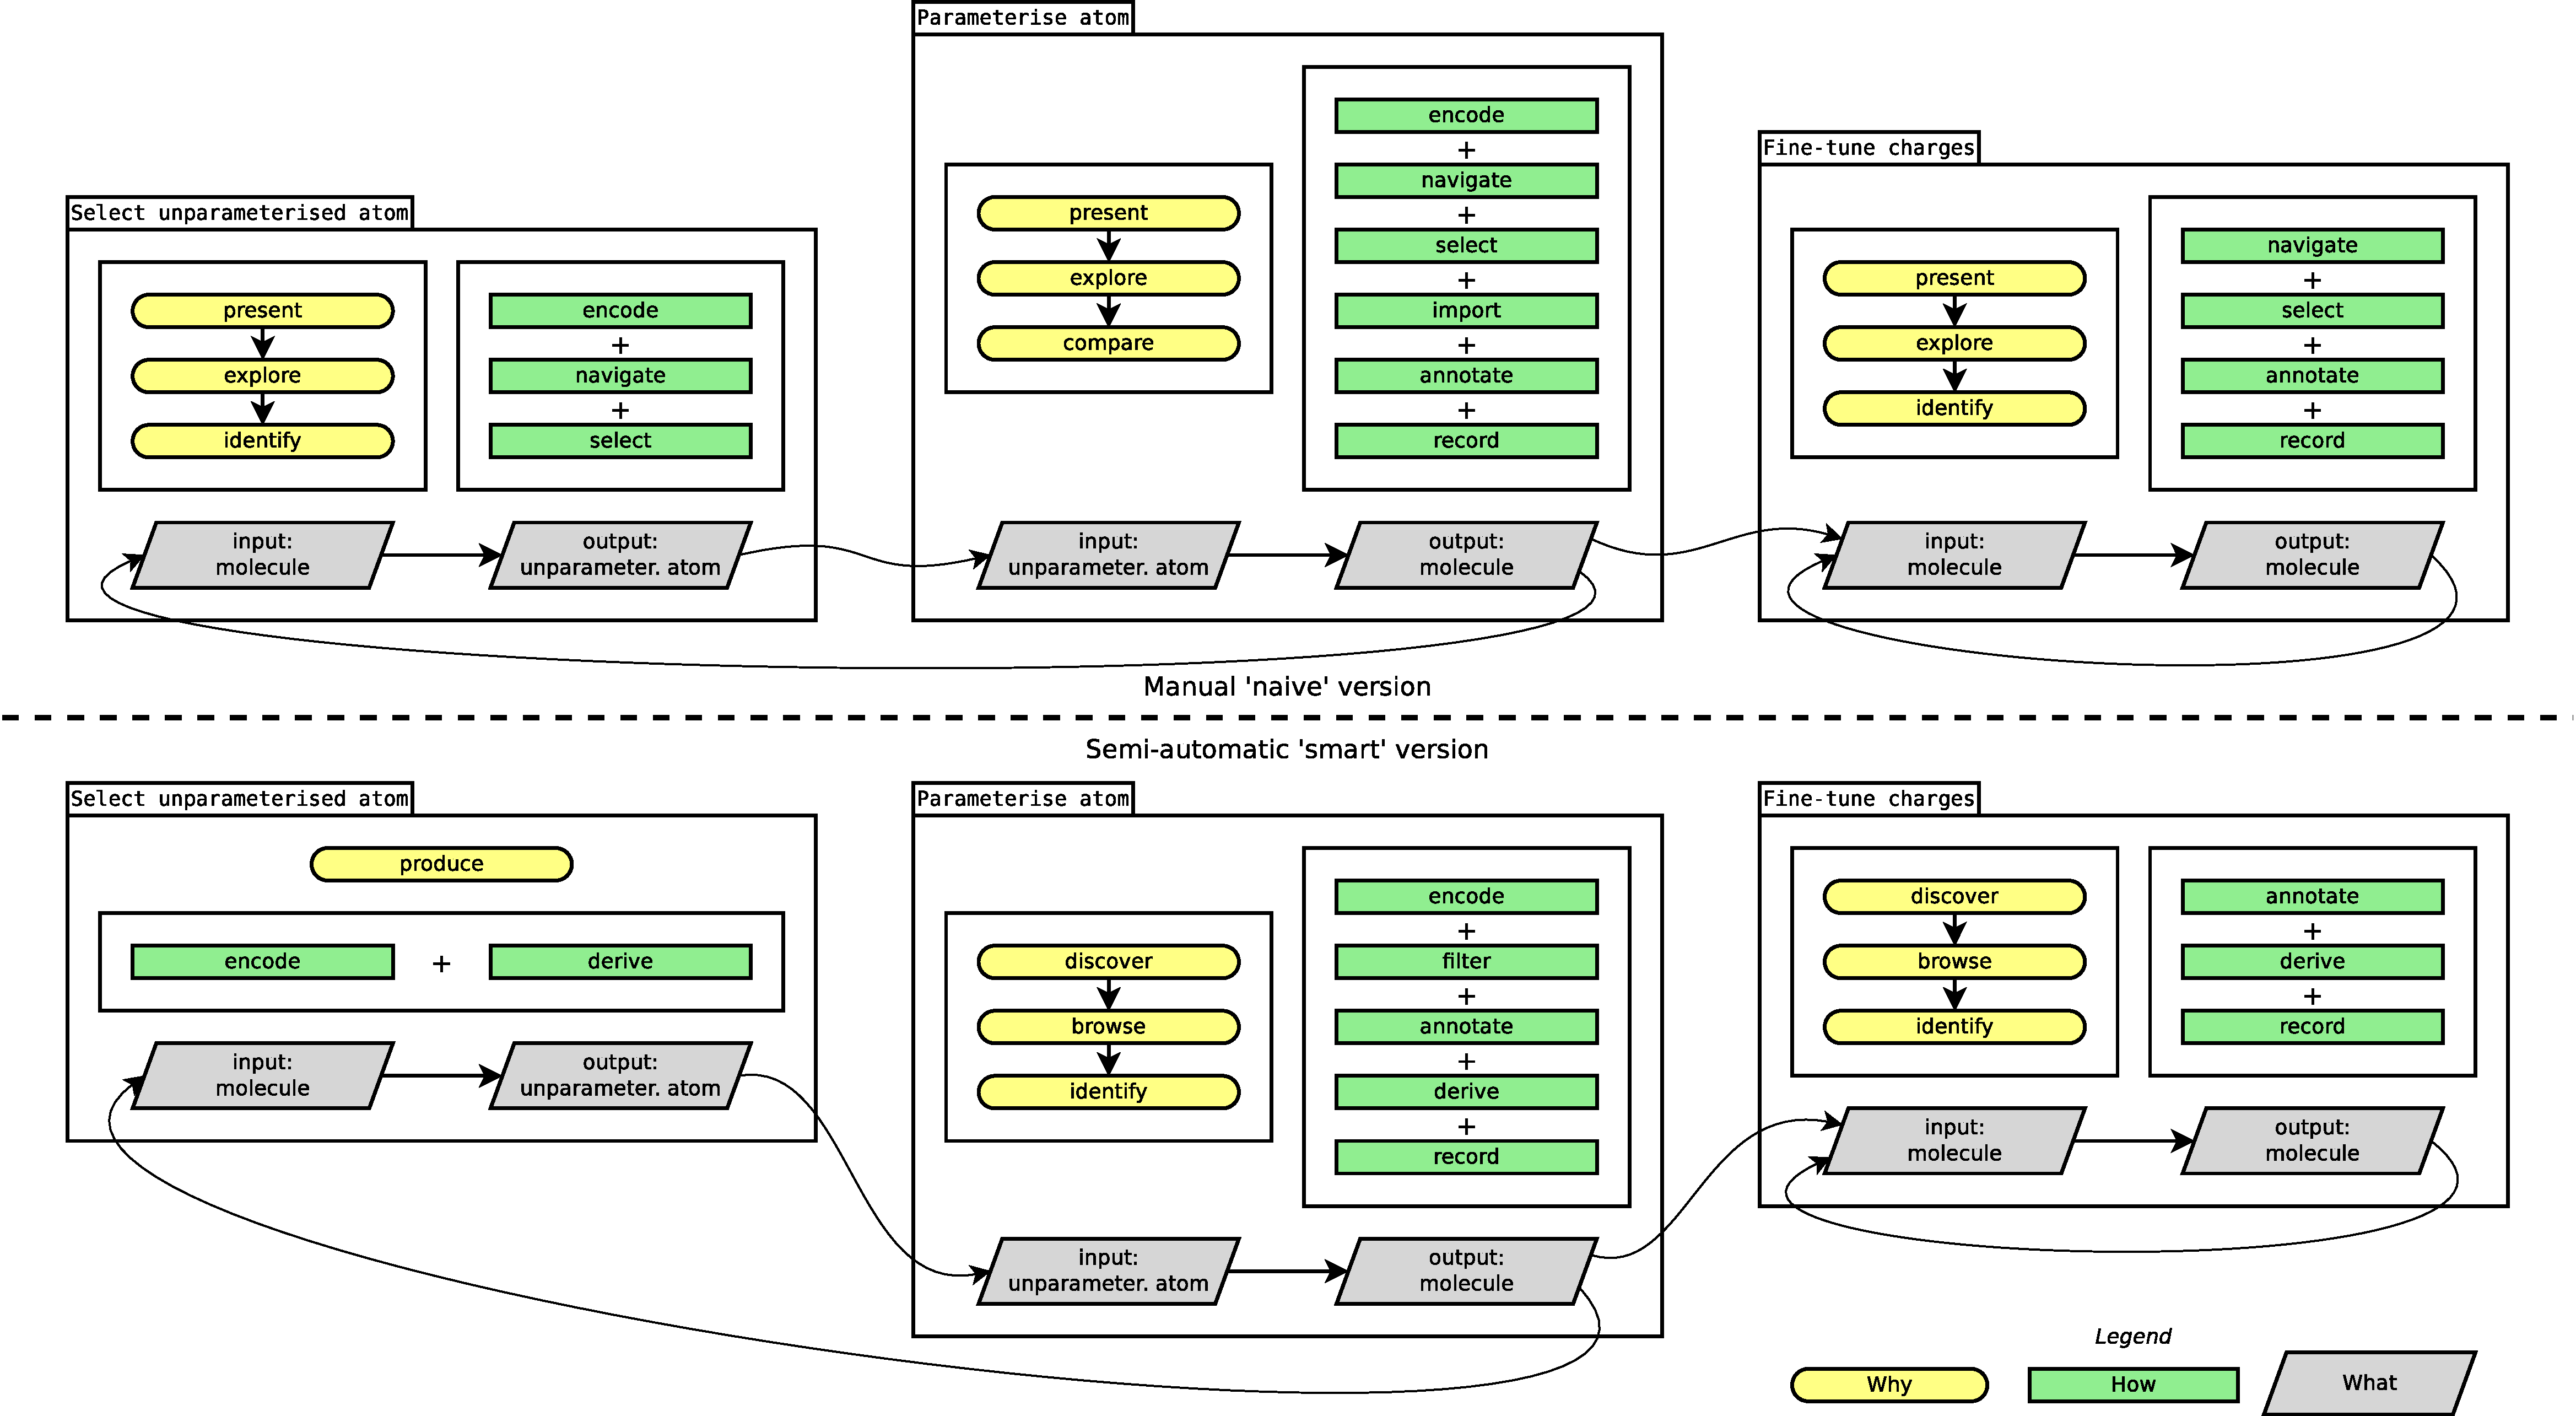
\includegraphics[width=\textwidth]{img/complete_typology.pdf}
\caption{Brehmer-Munzner Typologies of the two different interaction designs.}
\figlab{id_typologies}
\vspace{-2cm}
\end{center}
\end{figure}

These typologies clearly outline the differences between the two implementations. While the naive version is mainly concerned with presenting things to the user and user exploration,the user is mainly discovering (verifying) the system's proposals and browsing through them in the smart version. This means that, in the semi-automatic version, the user has easier access to the information, and can therefore make decisions earlier than in the naive version.

What is also clear in the typologies is the contrast in the number of different methods that is required to parameterise a molecule in the two versions. In every step of the process, the smart version requires less different methods than the naive one. This does not necessarily mean that the smart version will take less time to use, as the methods may need to be used more often. What it does mean, however, is that it will be easier to use the smart version, as less different methods need to be used and learned~\cite{sweller1994cognitive}~(see also \secref{id_learning}).
